\begin{table}
\begin{center}
\begin{tabular}{cc}
	\toprule
	\textbf{Input ingredient} & \textbf{Nearest neighbors}\\
	\midrule
	flour & warm water, egg yolk, nutmeg\\
	milk & melted butter, butter or margarine, eggs\\
	mozzarella & basil, pasta, freshly grated parmesan\\
	blueberries & frozen mixed berries, peaches, strawberries\\
	\bottomrule
\end{tabular}
\end{center}
\caption{Nearest neighbors (cosine distance) of some ingredients}
\label{nningredients}
\end{table}

We manually and subjectively evaluated our ingredient space by giving it an input ingredient and judging whether we consider the most similar vectors to be related gastronomically, where as a similarity measure we used the Cosine Distance, defined as $cos(\overright{u},\overright{v}) = \frac{<\overright{u},\overright{v}>}{\sqrt{||\overright{u}||\,||\overright{v}||}}$. For the most part, this works very well. When presented with an ingredient, the nearest neighbors seemed to ``fit well'' to it (Table~\ref{nningredients}).

Next, we manually looked at the nearest neighbors of composed recipes with recipes in the two recipe spaces. Our investigations seem to confirm our intuition: The \textbf{ComposedRecipes} space outperforms the primitive \textbf{BasicRecipes} space. When given, for example, ``water'', ``flour'', ``yeast'', and ``salt'', composing them leads to nearest neighbors such as ``home made mini bread'', ``Italian bread'', and ``french baguettes'' in \textbf{ComposedRecipes}, but ``pina colada baklava'', ``huckleberry cheesecake'', and ``honey-mint yogurt smoothie'' in \textbf{BasicRecipes}.

Quantitative evaluation of our work proved challenging. To automatically evaluate the quality of our vectors, we took all of our ingredients that are found in WordNet \citep{miller1995wordnet},
calculated the Cosine Distance between their vectors, and compared it with the JCN distance \citep[see (\ref{eq:jcn})\footnote{IC is the information content of a concept based on some corpus, LCS is the least common subsumer, i.e. the deepest node that subsumes both ingredients.}]{jiang1997semantic}
in WordNet, using the Brown corpus \citep{francis1979brown} as a seed corpus. As a comparism, we also compared it with the path distance in WordNet (see (\ref{eq:path})).

\begin{equation} \label{eq:path}
    Sim_{\mathrm{path}}(ing1, ing2) = \frac{1}{\mathrm{minpath}(ing1, ing2)}
\end{equation}
\begin{equation} \label{eq:jcn}
    Sim_{\mathrm{JCN}}(ing1, ing2) = \frac{1}{IC(ing1) + IC(ing2) - 2 * IC(LCS(ing1,ing2))}
\end{equation}

\begin{table}
    \begin{center}
        \begin{tabular}{ccc}
            \toprule
            \textbf{Cutoff at $n$} & \textbf{Path distance} & \textbf{JCN distance} \\
            \midrule
            10 & 0.63 & 0.53\\
            20 & 0.30 & 0.11\\
            50 & 0.06 & 0.13\\
            100 & 0.04 & 0.11\\
            \bottomrule
        \end{tabular}
    \end{center}
    \caption{Spearman's $\rho$ correlation between Cosine similarity and Path distance or JCN, respectively, at various cutoffs.}\label{tab:wordnet}
\end{table}

The Spearman correlation values for various cutoffs (using the most common $n$ ingredients) can be seen in Table~\ref{tab:wordnet}. None of them were significant with $p < 0.05$, but that is not too surprising: In WordNet, words are arranged according to their actual hierarchy, while our space attempts to represent how they are used in cooking, which could be (and is assumed to be) very different. For example, if \textit{butter} and \textit{olive oil} were used interchangeably in recipes, they would be very close in our space, but not in WordNet, because \textit{olive oil} is infact something very different from \textit{butter}.

\begin{figure}
    \begin{center}
        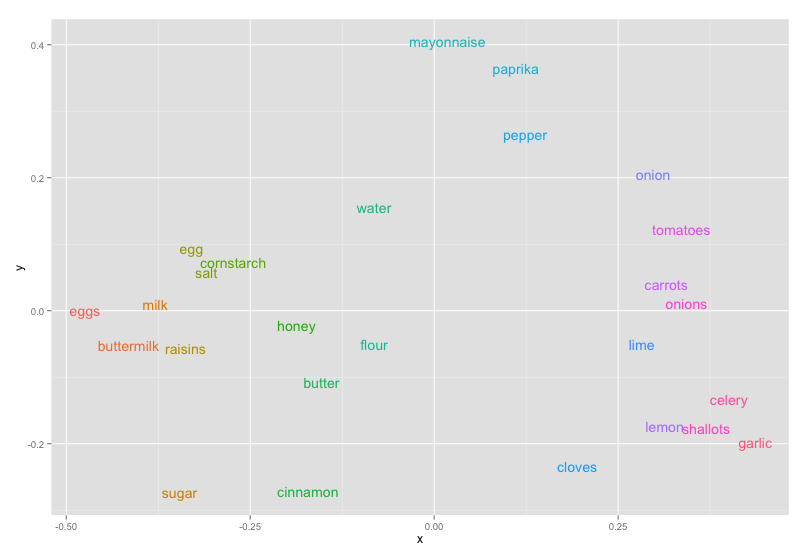
\includegraphics[scale=0.35]{toprainbow.png}
    \end{center}
    \caption{2D projection of ingredients}\label{fig:topsomething}
\end{figure}

\begin{figure}
    \begin{center}
        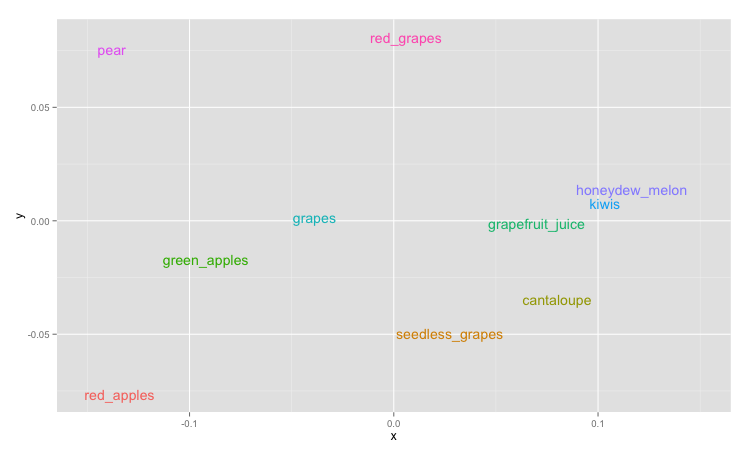
\includegraphics[scale=0.35]{grapes_final.png}
    \end{center}
    \caption{2D projection of the 10 nearest neighbors of ``grapes''}\label{fig:grapes}
\end{figure}

A 2D projection of some top ingredients from our space (plotted using the R library LSAfun \citep{LSAfun} with the Multidimensional Scaling (MDS) method), can be seen in Figure~\ref{fig:topsomething}. It can be seen that some similar ingredients cluster together: The spices ``paprika'' and ``pepper'' together on the top, vegetables on the middle right, and mostly sweet or neutral items on the left side of the plot (``sugar'', ``honey'', ``raisins'').

In Figure~\ref{fig:grapes}, the nearest neighbors of ``grapes'' were plotted using the same technique. It can be seen that all grape-related vectors are fairly close to each other, followed by other fruits and a fruit juice.
